\documentclass[a4paper,12pt]{book}
\usepackage[utf8]{inputenc}

\usepackage{rachwidgets}


\newcommand{\laClass}       {CS 211}
\newcommand{\laSemester}    {Spring 2017}
\newcommand{\laChapter}     {5.1}
\newcommand{\laType}        {Exercise}
\newcommand{\laPoints}      {5}
\newcommand{\laTitle}       {Intro to Combinatorics}
\newcommand{\laDate}        {Jan 16, 2018}
\setcounter{chapter}{5}
\setcounter{section}{1}
\addtocounter{section}{-1}
\newcounter{question}

\toggletrue{answerkey}
\togglefalse{answerkey}


\title{}
\author{Rachel Singh}
\date{\today}

\pagestyle{fancy}
\fancyhf{}

\lhead{\laClass, \laSemester, \laDate}

\chead{}

\rhead{\laChapter\ \laType\ \iftoggle{answerkey}{ KEY }{}}

\rfoot{\thepage\ of \pageref{LastPage}}

\lfoot{\scriptsize By Rachel Singh, last updated \today}

\renewcommand{\headrulewidth}{2pt}
\renewcommand{\footrulewidth}{1pt}

\begin{document}




\footnotesize
~\\ 
\textbf{\laChapter\ \laType: } In-class exercises are meant to introduce you to a new topic
and provide some practice with the new topic. Work in a team of up to 4 people to complete this exercise.
You can work simultaneously on the problems, or work separate and then check your answers with each other.
Completion score is given for this assignment.

~\\
Team:\\
(1) \tab[6cm] (2) \\
(3) \tab[6cm] (4)

\hrulefill
\normalsize 


\notonkey{
    \section{\laTitle}

    Combinatorics are counting problems, asking how many different combinations
    or outcomes there can be given some input(s), and when selecting a certain
    amount of items. These problems differ in how you solve them based on
    the type of structure.

    \begin{intro}{Types of structures}
        \begin{center}
            \begin{tabular}{l | c | c | c }
                \textbf{}
                    & \textbf{Repeats allowed?}
                    & \textbf{Order matters?}
                \\ \hline
                Ordered list
                    & yes
                    & yes

                \\ \hline
                Unordered list
                    & yes
                    & no
                \\ \hline
                Permutations
                    & no
                    & yes
                \\ \hline
                Sets
                    & no
                    & no
            \end{tabular}
        \end{center}
    \end{intro}

    \stepcounter{question}
    \begin{questionNOGRADE}{\thequestion}
        \underline{Identify the structure type} for each of the following problems.
        You DON'T need to solve the problems.

        \begin{enumerate}
            \item[a.]   You want to throw a birthday party at your favorite restaurant,
                        but you can only book 8 seats. You have 11 friends to choose from.
                        How many different groups of friends could attend your birthday party?
                        \begin{center}
                            Repetitions allowed? \tab Order matter? \tab What structure?
                        \end{center}
                        
            \item[b.]   There are only 4 bags of chips left at the sandwich shop:
                        Nacho, ranch, garden, and potato. You and your friend both
                        want chips. If you're selecting first for your friend
                        and then for yourself, how many ways are there to get chips?
                        \begin{center}
                            Repetitions allowed? \tab Order matter? \tab What structure?
                        \end{center}
        \end{enumerate}
    \end{questionNOGRADE}

    \begin{questionNOGRADE}{\thequestion\ (continued)}
        \underline{Identify the structure type} for each of the following problems.
        You DON'T need to solve the problems.

        \begin{enumerate}
            \item[c.]   A student is purchasing colored pens to use for each of their four classes.
                        First they choose a pen for Discrete Math, then for English, then for
                        Physics, and then for Programming. They can choose from the colors
                        red, orange, yellow, green, blue, or purple.
                        \begin{center}
                            Repetitions allowed? \footnote{Nothing in the problem specifies that it isn't, and choosing pens in and of itself isn't generally a ``is this unique?'' type of problem.}
                            \tab Order matter? \tab What structure?
                        \end{center}
                        
            \item[d.]   You're filling your plate with food at a buffet. As you go down the buffet line,
                        you might get more than one dessert... just because. If there are 5 main meal items
                        and 1 dessert item, how many dinner combinations can you make if you have space for 3 items?
                        \begin{center}
                            Repetitions allowed?
                            \tab Order matter? \tab What structure?
                        \end{center}
        \end{enumerate}
    \end{questionNOGRADE}

    \hrulefill
    
    \stepcounter{question}
    \begin{questionNOGRADE}{\thequestion}

        We have a pool of four people, Andrew, Bob, Carly, Diane, and two prizes will be distributed
        between two of these people.
        \footnote{Based on Practice Problem 2 from Discrete Mathematics, Ensley \& Crawley}

        \begin{enumerate}
            \item[a.] Assuming that prize \#1 and prize \#2 are different, list out
            all the ways the prizes can be distributed (i.e., permutations).

            \textit{Example: (A, A), (A, B), (B, A), ...}

            \item[b.] Assuming that prize \#1 and price \#2 are both the same,
            list out all the ways the prizes can be distributed (i.e., sets).

            \textit{Note: \{A, B\} and \{B, A\} would be considered the same.}
        \end{enumerate}
        
    \end{questionNOGRADE}

    \newpage

    \stepcounter{question}
    \begin{questionNOGRADE}{\thequestion}

        All possible outcomes of rolling a red 6-sided die and a green 6-sided die,
        in an organized way is given in the table. For the given set of data, answer the questions.
        \footnote{Based on Exercise 5.1 \#6 from Discrete Mathematics, Ensley \& Crawley}
        ~\\

        \begin{tabular}{ l | c c c c c c }
            & Green 1 & Green 2 & Green 3 & Green 4 & Green 5 & Green 6 \\ \hline
            Red 1 & (1,1) & (1,2) & (1,3) & (1,4) & (1,5) & (1,6) \\
            Red 2 & (2,1) & (2,2) & (2,3) & (2,4) & (2,5) & (2,6) \\
            Red 3 & (3,1) & (3,2) & (3,3) & (3,4) & (3,5) & (3,6) \\
            Red 4 & (4,1) & (4,2) & (4,3) & (4,4) & (4,5) & (4,6) \\
            Red 5 & (5,1) & (5,2) & (5,3) & (5,4) & (5,5) & (5,6) \\
            Red 6 & (6,1) & (6,2) & (6,3) & (6,4) & (6,5) & (6,6) \\
            
        \end{tabular}

        \begin{enumerate}
            \item[a.]   Of the listed outcomes, how many are ``doubles''
                        (both dice have the same value)? What percentage of
                        total outcomes does this represent?
                        (You can write it as a fraction)

            \item[b.]   How many are doubles \textit{and} have the sum
                        of two dice values less than 4?
                        (You can write it as a fraction)

            \item[c.]   How many have a 5 on exactly one of the dice?

            \item[d.]   How many have a 5 on at least one of the dice?
        \end{enumerate}
        
    \end{questionNOGRADE}

    \hrulefill

    \stepcounter{question}
    \begin{questionNOGRADE}{\thequestion}

        Identify all possible outcomes for the following:

        \begin{enumerate}
            \item[a.]   All possible outcomes if you flip one coin.
            
            \item[b.]   All possible outcomes if you flip two coins together.
            
            \item[c.]   All possible outcomes if you flip three coins together.
        \end{enumerate}
        
    \end{questionNOGRADE}

    \newpage

    \stepcounter{question}
    \begin{questionNOGRADE}{\thequestion}

        The following tree diagrams all possible outcomes when tossing a penny,
        a nickel, and a dime together. Given this tree, answer the following questions
        \footnote{Based on Exercise 5.1 \#8 from Discrete Mathematics, Ensley \& Crawley}

        \begin{center}
            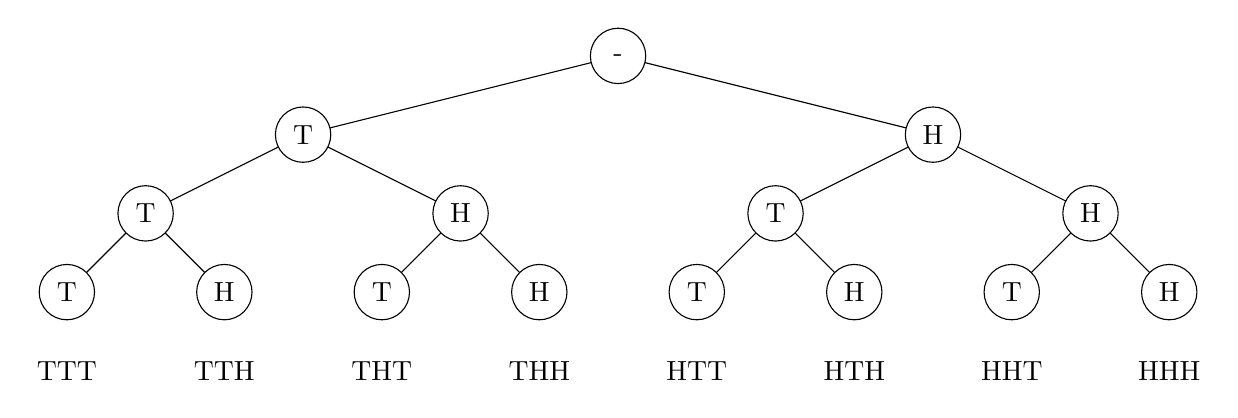
\begin{tikzpicture}
                \draw (-7,1) -- (-6,2);     \node at (-7,0) {TTT};
                \draw (-5,1) -- (-6,2);     \node at (-5,0) {TTH};
                \draw (-3,1) -- (-2,2);     \node at (-3,0) {THT};
                \draw (-1,1) -- (-2,2);     \node at (-1,0) {THH};
                
                \draw (-6,2) -- (-4,3);
                \draw (-2,2) -- (-4,3);
                
                \draw (-4,3) -- (0,4);
                
                \draw (1,1) -- (2,2);     \node at (1,0) {HTT};
                \draw (3,1) -- (2,2);     \node at (3,0) {HTH};
                \draw (5,1) -- (6,2);     \node at (5,0) {HHT};
                \draw (7,1) -- (6,2);     \node at (7,0) {HHH};
                
                \draw (6,2) -- (4,3);
                \draw (2,2) -- (4,3);
                
                \draw (4,3) -- (0,4);
                
                \filldraw[fill=white] (0,4) circle (10pt) node{-};
                
                \filldraw[fill=white] (-4,3) circle (10pt) node{T};
                \filldraw[fill=white] (4,3) circle (10pt) node{H};
                
                \filldraw[fill=white] (-6,2) circle (10pt) node{T};
                \filldraw[fill=white] (-2,2) circle (10pt) node{H};
                
                \filldraw[fill=white] (6,2) circle (10pt) node{H};
                \filldraw[fill=white] (2,2) circle (10pt) node{T};
                
                \filldraw[fill=white] (-7,1) circle (10pt) node{T};
                \filldraw[fill=white] (-5,1) circle (10pt) node{H};
                
                \filldraw[fill=white] (-3,1) circle (10pt) node{T};
                \filldraw[fill=white] (-1,1) circle (10pt) node{H};
                
                \filldraw[fill=white] (7,1) circle (10pt) node{H};
                \filldraw[fill=white] (5,1) circle (10pt) node{T};
                
                \filldraw[fill=white] (3,1) circle (10pt) node{H};
                \filldraw[fill=white] (1,1) circle (10pt) node{T};
            \end{tikzpicture}
        \end{center}

        \begin{enumerate}
                \item[a.]   Of the outcomes shown, for how many does
                            the result on the penny match the result on the dime?

                \item[b.]   Which is more likely, that the result on the penny
                            matches the result on the dime, or that they do not match?

                \item[c.]   For how many of the outcomes do all three coins match?

                \item[d.]   For how many of the outcomes do exactly two of the coins match?

                \item[e.]   For how many outcomes is the number of tails less than the number of heads?
        \end{enumerate}
        
    \end{questionNOGRADE}

}{
    ~\\ Question 1 a:   Repetitions aren't allowed, order doesn't matter: Is a set (combination).

    ~\\ Question 1 b:   Repetitions aren't allowed, order does matter: Is a permutation.

    ~\\ Question 1 c:   Repetitions are allowed, order does matter: Is an ordered list.

    ~\\ Question 1 d:   Repetitions are allowed, order doesn't matter: Is an unordered list.

    ~\\ Question 2 a:
                    \begin{center}
                        \begin{tabular}{c | c c c c}
                            & A & B & C & D \\ \hline
                            A & (A,A) & (A,B) & (A,C) & (A,D)
                            \\
                            B & (B,A) & (B,B) & (B,C) & (B,D)
                            \\
                            C & (C,A) & (C,B) & (C,C) & (C,D)
                            \\
                            D & (D,A) & (D,B) & (D,C) & (D,D)
                        \end{tabular}
                    \end{center}

    ~\\ Question 2 b:
                    \begin{center}
                        \begin{tabular}{c | c c c c}
                            & A & B & C & D \\ \hline
                            A & (A,A) & (A,B) & (A,C) & (A,D)
                            \\
                            B &  & (B,B) & (B,C) & (B,D)
                            \\
                            C &  &  & (C,C) & (C,D)
                            \\
                            D &  &  &  & (D,D)
                        \end{tabular}
                    \end{center}

    ~\\ Question 3 a:   There are 36 total outomes, and 6 total doubles. 6/36 = 1/6

    ~\\ Question 3 b:   Double with a sum of less than 4 include just (1,1), so 1/36.

    ~\\ Question 3 c:   (1,5), (5,1), (5,2), (5,3), (5,4), (5,5), (5,6), (6,5).
                        So, 8

    ~\\ Question 3 d:   (1,5), (5,1), (5,2), (5,3), (5,4), (5,6), (6,5).
                        So, 7

    ~\\ Question 4 a:   H, T
    
    ~\\ Question 4 b:   H-H, H-T, T-H, T-T
    
    ~\\ Question 4 c:   H-H-H, H-H-T, H-T-H, H-T-T, T-H-H, T-H-T, T-T-H, T-T-T

    ~\\ Question 5 a:   4
    
    ~\\ Question 5 b:   They are equally likely
    
    ~\\ Question 5 c:   2
    
    ~\\ Question 5 d:   6
    
    ~\\ Question 5 e:   4
}

    



\end{document}

